\subsection{Projekt systemu mulitplayer}
Do utworzenia systemu Multiplayer został użyty Framework Photon Unity 3D Networking często nazywany PUN. 
Photon udostępnia również chmurę, na której znajduje się nasza aplikacja, dzięki temu nie jest wymagane użycie innego, zewnętrznego serwera. 
\begin{figure}[H]
	\center
	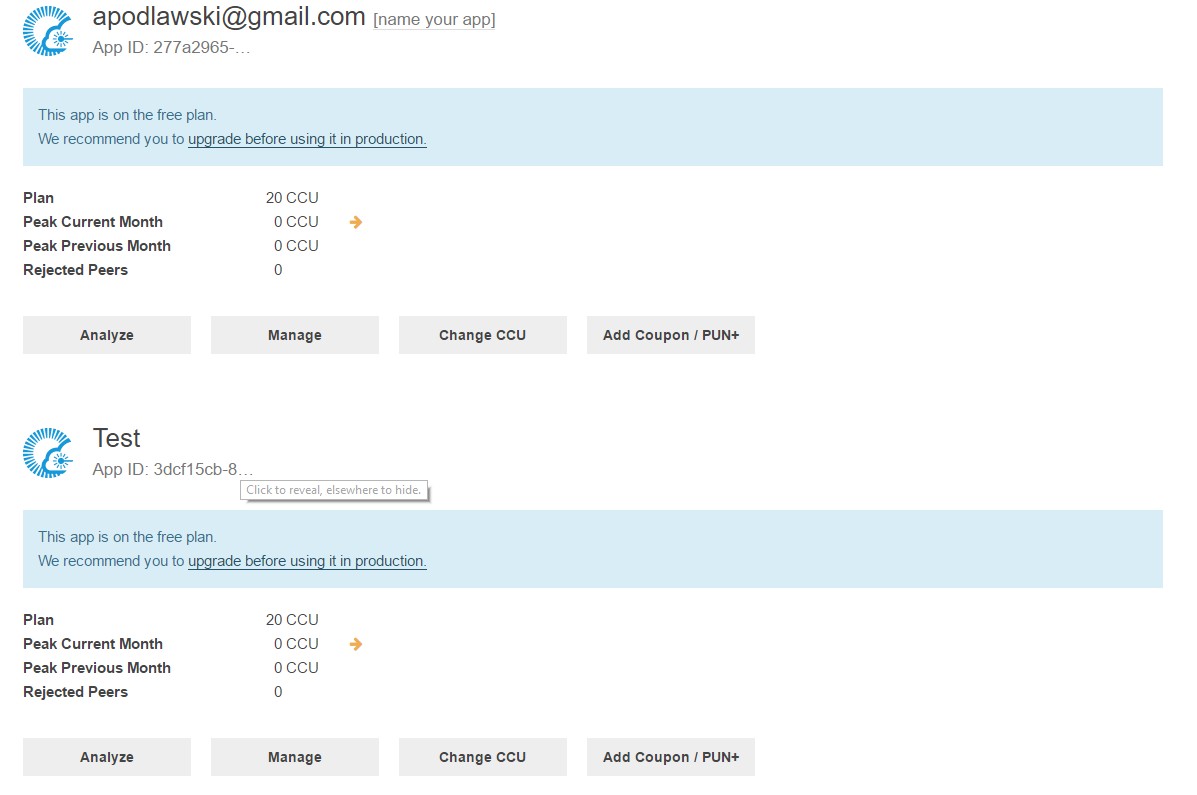
\includegraphics[width=\textwidth]{maszyny.png}
	\caption{Serwery udostępniane przez framework Photon, na których znajdują się nasze środowiska testowe oraz produkcyjne}
\end{figure}
Gracze po włączeniu gry automatycznie dołączają do rozgrywki. Maksymalnie do jednej rozgrywki może połączyć się trzech graczy. Jeżeli do serwera dołączy czwarty gracz, zostanie utworzony kolejny pokój gry, a wszyscy kolejni użytkownicy będą mogli się z nim połączyć, dopóki nie zostanie osiągnięty limit osób. 
Każda postać jest unikatowa i poszczególny gracz może sterować tylko jedną z nich. Jeśli jeden gracz opuści grę, kolejny po dołączeniu zajmie jego miejsce. 